\documentclass[a4paper,12pt]{report}
\usepackage{graphicx}  % For including graphics
\usepackage{hyperref}  % For hyperlinks
\usepackage{listings}  % For code snippets
\usepackage{tocbibind} % For adding ToC to the table of contents
\usepackage{titlesec}  % For customizing titles
\usepackage[ngerman]{babel}
\usepackage{wasysym}


\usepackage{geometry}
\geometry{
    top=1in,
    left=1in,
    right=1in,
    bottom=1in
}


\titleformat{\chapter}[block]   % Set chapter format to block style (both on same line)
{\normalfont\huge\bfseries}     % Format for the chapter number and title
{\thechapter}                   % Shows the chapter number followed by a dot
{0.5em}                         % Space between the chapter number and title
{}                              % Formatting for the chapter title (leave empty)

\renewcommand{\contentsname}{Inhaltsverzeichnis}
\renewcommand{\listtablename}{Tabellenverzeichnis}
\renewcommand{\listfigurename}{Abbildungsverzeichnis}
\renewcommand{\lstlistlistingname}{Code-Ausschnitte}
\renewcommand{\abstractname}{Zusammenfassung}
\renewcommand{\chaptername}{Kapitel}

\begin{document}

% Title Page
    \begin{titlepage}
        \centering
        \textit{Berner Fachhochschule}\\[0.2em]
        \textit{BTI3031 Project 1}
        \vfill
        {\huge \textbf{AI-Aided Caches-n-Logs Monitoring-n-Wiping Daemon}}\\[4em]
        {\large Luca Scherer, Janic Scherer, Luca Ammann }\\[0.5em]
        \begin{tabular}{ll}
        \textbf{Betreuer:}\hspace{0.5em}Dr. Simon Kramer \\
        \end{tabular}

        \vfill
        \textit{\today}
    \end{titlepage}

% Abstract
    \begin{abstract}
        \ldots
    \end{abstract}

% Table of Contents
    \tableofcontents
    \listoftables
    \listoffigures
    \lstlistoflistings

% Main Content


    \chapter{Einleitung}


    \section{Ausgangssituation}


    \section{Projektziel}


    \section{Prioritäten}


    \chapter{Spezifikation}

    \newpage
    \section{Systemabgrenzung}

    \subsection{Systemumgebung}

    \subsubsection{Komponenten}


    \begin{figure}[h]
        \centering
        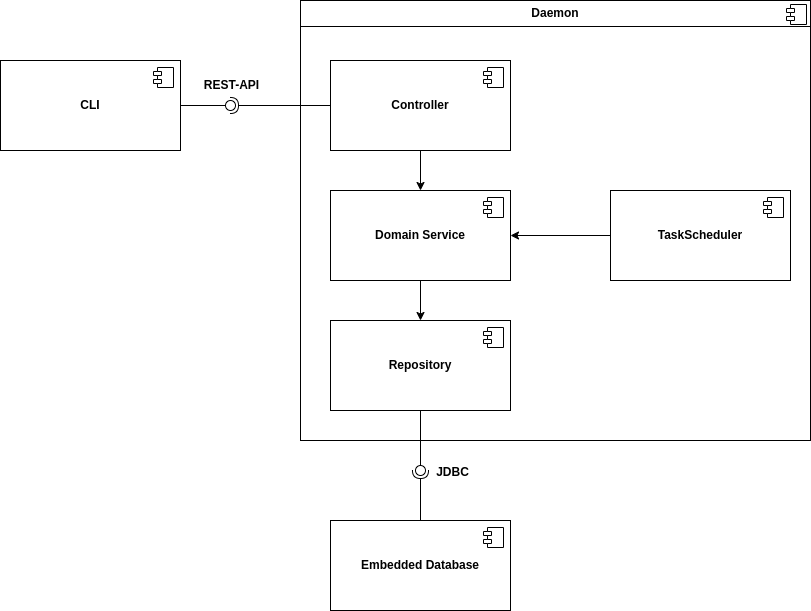
\includegraphics[width=1\textwidth]{assets/comp-diag-aclom}
        \caption{UML Komponentendiagramm}
        \label{fig:comp-diag}
    \end{figure}
    
    \textnormal{Das System besteht aus zwei Hauptkomponenten, welche als eigene Laufzeiteinheiten ausgeführt werden.
    Die CLI wird ad hoc gestartet und dient als Benutzerschnittstelle.
    Der Daemon läuft nach dem Start im Hintergrund und führt periodisch Befehle aus. Ausserdem stellt er der
    CLI eine REST-Schnittstelle zur Verfügung.
    Ein eingebettetes Datenbanksystem speichert die Applikationsdaten.}

    \begin{table}[h!]
        \centering
        \setlength{\leftmargini}{0.4cm}
        \begin{tabular}{|p{2.5cm}|p{5.5cm}|p{3cm}|}
            \hline
            \textbf& \textbf{Zweck} & \textbf{Technologien (primär)} \\
            \hline
            \textbf{CLI} & {Stellt eine Kommandozeilen-Benutzerschnittstelle zur Verfügung.} & Java, Spring (Shell) \\
            \hline
            \textbf{Controller} & Implementiert die Endpunkte der REST-Schnittstelle & Java, Spring (Data) \\
            \hline
            \textbf{Domain Service} & Applikationslogik & Java, Spring \\
            \hline
            \textbf{Task Scheduler} & Führt Funktionen periodisch aus & Java, Spring \\
            \hline
            \textbf{Repository} & Stellt den Zugang zu den persisiterten Daten zur Verfüfung & Java, Spring (Data) \\
            \hline
            \textbf{Embedded Database} & Speichert Applikationsdaten & SQLite \\
            \hline
        \end{tabular}
        \caption{Beschreibung der Komponenten}\label{tab:table3}
    \end{table}

    \newpage

    \subsection{Prozessumgebung}

    \newpage
    \section{Anforderungen}
    \subsection{Funktionale Anforderungen}

    \begin{table}[h!]
        \centering
        \setlength{\leftmargini}{0.4cm}
        \begin{tabular}{|c|p{10cm}|}
            \hline
            \textbf{ID} & FR-001 \\ \hline
            \textbf{Anforderung} & Suche von Log und Cache Files \\ \hline
            \textbf{Beschreibung} & In einem bestimmten Verzeichnis durchsucht das System jegliche Dateinamen inkl. dieser in Unterordnern, um Log \& Cache Files zu identifizieren.  \\ \hline
            \textbf{Akzeptanzkriterien} &
            \begin{itemize}
                \item Der deamon kann via CLI gestartet werden.
                \item Alle Konfigurationen und Aktionen des deamon sind via CLI verfügbar.
            \end{itemize}
            \\ \hline
        \end{tabular}
        \caption{Funktionale Anforderung FR-001}\label{tab:table2}
    \end{table}


    \newpage
    \subsection{Grenz- und Vorbedingungen}
    TODO systemunabhängigkeit, evtl. erweiterbarkeit des ui (kommunikation zwischen cli und deamon),
    Folgend 2 eher nicht funktionale Anforderungen

    \begin{table}[h!]
        \centering
        \setlength{\leftmargini}{0.4cm}
        \begin{tabular}{|c|p{10cm}|}
            \hline
            \textbf{ID} & FR-001 \\ \hline
            \textbf{Anforderung} & Hintergrundprozess mit periodischem Task (deamon) \\ \hline
            \textbf{Beschreibung} & Das System muss einen Hintergrundprozess implementieren, der periodisch Aktionen durchführen kann. \\ \hline
            \textbf{Akzeptanzkriterien} &
            \begin{itemize}
                \item Nach dem Start des Prozesses, ist dieser für den Benutzer nicht mehr ersichtlich.
                \item Der Hintergrundprozess ist erweiterbar, sodass dieser periodisch und autonom Aktionen durchführen kann.
            \end{itemize}
            \\ \hline
        \end{tabular}
        \caption{Funktionale Anforderung FR-001}\label{tab:table}
    \end{table}

    \begin{table}[h!]
        \centering
        \setlength{\leftmargini}{0.4cm}
        \begin{tabular}{|c|p{10cm}|}
            \hline
            \textbf{ID} & FR-002 \\ \hline
            \textbf{Anforderung} & Benutzerschnittstelle via Konsole (CLI) \\ \hline
            \textbf{Beschreibung} & Mit dem laufenden deamon soll via Konsole interagiert werden können \\ \hline
            \textbf{Akzeptanzkriterien} &
            \begin{itemize}
                \item Der deamon kann via CLI gestartet werden.
                \item Alle Konfigurationen und Aktionen des deamon sind via CLI verfügbar
            \end{itemize}
            \\ \hline
        \end{tabular}
        \caption{Funktionale Anforderung FR-002}\label{tab:table2}
    \end{table}

    \section{Usability}

    \subsection{Personas}

    \subsection{Storyboard}

    \subsection{UX-Prototyping}


    \chapter{Implementierung}


    \section{Architektur}


    \section{Prozesse}
    \url{https://www.ganttlab.com} \\
    \url{https://www.hermes.admin.ch/de/projektmanagement/verstehen/ubersicht-hermes/methodenubersicht.html}


    \chapter{Bereitstellung/Integration}


    \section{Lizenzierung}


    \section{Installationshandbuch \& Skript}


    \section{Benutzerhandbuch}


    \chapter{Fazit}


    \section{Diskussion}


    \section{Zusammenfassung}


    \section{Zukünftige Arbeiten}
    \url{https://doi.org/10.1145/3664811}


    \chapter{Glossar}


    \chapter{Index}


    \chapter{Bibliografie}


    \chapter{Anhang}


    \section{Facsimile der Projektbeschreibung}


    \section{Erklärung zur Urheberschaft}

\end{document}
